\chapter{Introduction}

JavaScript (JS), the \emph{de facto} language of the web, has recently gained much
popularity among researchers and practitioners alike. In particular, due to the
highly dynamic nature of the language, there is a growing interest in observing
the behavior of JS programs. For instance, run-time monitoring is being used for
widely different purposes, such as gathering empirical data regarding the
dynamic behavior of web applications~\cite{behavior_js}, automatically
extracting benchmarks from web applications~\cite{Richards:2011}, and enforcing
access permission contracts~\cite{Heidegger:2012}.

Common profiling tasks in JS, such as intercepting all object operations or
function calls, are difficult to achieve in a portable and efficient
manner. A popular approach consists of modifying a production virtual machine
(VM). While this approach guarantees a high level of compliance with the source
language, it suffers from some important drawbacks. Most modern JS
implementations are production-quality VMs that are optimized for performance
and thus difficult to modify. Generally, this approach also binds the profiling
system to a single VM, and therefore greatly limits the portability of the
approach. Moreover, modifications to the VM codebase must evolve as the VM is
being developed upstream, which can happen at a rapid pace. As a result,
many attempts to modify a JS VM are punctual efforts that are abandoned shortly
thereafter. 

The most popular alternative approach for instrumenting JS programs consists of
implementing an \textit{ad hoc} source-to-source translator and runtime
library tailored to the problem at hand. While this approach is easier to maintain and
more portable than instrumenting a VM, implementing a correct source-to-source
transformation is deceptively difficult in practice, even for seemingly simple
tasks. For instance, instrumenting all object creations also requires
instrumenting all function calls because any function call could potentially be
a call to \kw{Object.create} through an alias. Other dynamic constructs in JS,
such as \kw{eval}, are notoriously difficult to instrument while guaranteeing
that the observed behavior of the program will remain unaffected. Also, JS
programs can easily redefine core operations from \kw{Object} and \kw{Array}.
Such modifications are difficult to handle. A profiler that is unaware of such
redefinitions could behave incorrectly, or worse, cause a change in the
observed behavior of the profiled program. Finally, the profiler code itself
must maintain various invariants. For example, instrumentations that rely on
extending existing objects with new properties must take proper care not to
leak information that is visible to user code by introspection (e.g., by
iterating over all properties of an object\footnote{Marking properties as
non-iterable is not sufficient in general, since
\kw{Object.getOwnPropertyNames} will return all property names, irrespective of
their iterable nature.}).

Both VM instrumentation as well as source-to-source transformations can have
unexpected performance costs. VM instrumentation often settles for
modifying a simple non-optimizing interpreter to avoid the additional
complexity of instrumenting a commercial Just-In-Time (JIT) compiler. The
performance hit incurred by disabling the JIT compiler in a modern JS
implementation is significant, often an order of magnitude or more. Second,
while source-to-source transformations can benefit from the full range of
optimizations performed by the JIT, a naive transformation often results in a
similar slowdown.

In this dissertation, we present an alternative technique for run-time
monitoring of JS applications based on \emph{virtual machine layering}. Virtual
machine layering consists of exposing low-level internal operations performed
by the VM through various abstraction layers. Specifically, our approach uses a
flexible \emph{object model} as a basis to build the abstraction layers.  A JS
application is then transformed to make use of these abstractions. Because this
transformation is performed during the execution, the resulting framework can
be viewed as a metacircular VM written on top of a host VM for the source
language. This approach has three main advantages. First, exposing low-level
operations provides a good compromise between the portability offered by
source-to-source translations and the expressiveness of VM modifications. For
instance, profilers can easily extend or redefine the low-level operations to
accomplish their specific tasks. Second, by exposing low-level operations in a
separate layer, our approach can prevent interference between monitoring code and application 
code. This is achieved by ensuring that application code only manipulates objects
through \emph{proxies}, which provide a form of sandboxing over the native
objects provided by the host VM. Finally, the metacircular VM can leverage fast
operations provided by the underlying host VM to reduce the overhead of the
transformation. This is achieved by (i) letting the host VM execute operations
for which no abstraction is necessary, and (ii) providing abstractions that use
or support the operations that are efficiently implemented by the host VM.
Reusing complex primitive operations from the host VM also greatly reduces the
development effort required to provide a fully compliant VM implementation.

Photon, our prototype implementation of this technique, uses a single primitive
operation, message-sending, to reify low-level operations such as object
operations and function calls. The use of the message-sending primitive
provides a simple and dynamic mechanism to instrument and even redefine the
behavior of a reified operation. For instance, a profiler could intercept all
calls by providing a wrapper function for Photon's \kw{call} primitive
operation. In order to offset the cost of the message-sending mechanism, Photon
implements a {\it send cache} optimization. This optimization allows the behavior of
a message send (e.g., a property access) to be specialized at a given program
point. This caching optimization is crucial to obtain a good performance in
practice, making Photon on average 19\% faster than a commercial interpreter
while providing a much higher degree of flexibility and dynamism. Because the
caching mechanism itself relies on message sends to perform the
specialization, it is sufficiently flexible to allow instrumentations that
specialize the operations that they redefine in order to improve performance.

This dissertation therefore shows that \emph{virtual machine layering} is a
competitive alternative approach to VM instrumentation for run-time monitoring
of object operations and function calls.

\section{Overview}

In a conventional JS setting, an application runs over a high-performance host
VM. In the case of a \emph{metacircular} VM, an additional VM layer is
inserted between the application and the host VM. This layer can be a
\emph{full} or a \emph{differential} implementation. In a full implementation,
the metacircular VM provides all functionalities of the source language. In a
differential setting, however, the metacircular VM only implements parts of
the required functionality, and delegates the remaining operations to the
underlying host VM. Our approach follows a differential strategy.
Object
 operations are handled by one of the layers introduced by
Photon while primitive operations are handled by the host VM.

This section discusses the objectives that guided the design decisions,
followed by an overview of the Photon VM and its components.

\subsection{Design goals}

Our design aims to achieve the following properties:
\begin{itemize}
    \item \textbf{Isolation}: The application is isolated to avoid any
        interference with instrumentation code, while still allowing an
        instrumentation to fully inspect and modify the application state.
    \item \textbf{Flexibility}: The semantics of object operations and function
        calls are exposed as methods so that they can be extended or
        completely redefined, as required by the instrumentation.
    \item \textbf{Dynamism}: The semantics of object operations and function
        calls can be redefined while the application is running to allow
        instrumentations to precisely control the start and duration
        of their monitoring (e.g., only after the startup phase of the application).
    \item \textbf{Abstraction}: Low-level details, mostly related to
        performance optimizations, are encapsulated by specific layers to
        simplify the definition of instrumentations.
    \item \textbf{Performance}:
        Since native features provided by the host VM are often implemented
        very efficiently, our implementation reuses them when possible (e.g.,
        the scope chain and control-flow operations). Furthermore, Photon
        leverages the performance of some host feature (e.g., fast global
        function calls) to perform optimizations that reduce the overhead
        introduced by the abstraction layers.
\end{itemize}

\subsection{Overview of the Components}

\begin{figure*}[tbp]
\begin{center}
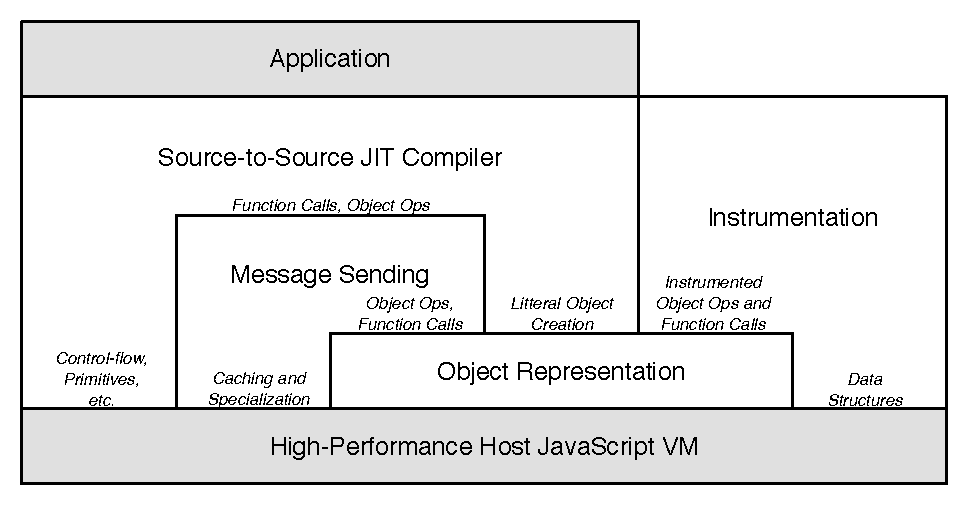
\includegraphics[width=.85\textwidth]{figures/architecture_simplified}
\caption{\label{fig:Architecture} Components of the Photon virtual machine}
\end{center}
\end{figure*}

Figure~\ref{fig:Architecture} shows a structural view of the components of the
layered VM implemented by Photon.

\paragraph{Source-to-Source Compiler.} The source-to-source compiler translates
the original JS code to use the runtime environment provided by
Photon.  Non-reified elements, such as control-flow operations as well as
primitive values and operations are preserved. Object operations and function
calls are translated to make use of the message sending layer. Literal object
creations are translated to use the object representation. The
source-to-source compiler is itself written in JS and is therefore available
at run-time. By staging it in front of every call to \kw{eval}, it effectively
provides a JIT compiler to Photon.

\paragraph{Message Sending.} Photon uses a message sending primitive to reify
low-level operations such as property accesses on objects and function calls.
These reified operations can then easily be overridden and redefined when
required, for example to profile the application or to specialize the behavior
of an operation. Photon itself makes use of this extra level of indirection for
performance by providing a caching mechanism at each site that performs a
message send, a form of memoization.

\paragraph{Object Representation.} In order to isolate the application from
the instrumentation and the host VM, Photon provides a virtualized
representation of objects (including functions). Each JS object in the
original application is represented in Photon by \emph{two} distinct objects:
a property container and a proxy. The property container corresponds to the
original object, and acts as storage for all properties that are added to an
object. For performance reasons, the property container object is a native JS
object provided by the host VM. This allows Photon to leverage the efficient
property access mechanism provided by the host VM.

% Erick clarifications:
%   A separate host-level object with its own proxy serves as a global object
%   to isolate the application from the execution environment of Photon. The
%   host-level global object is reserved for optimization of reified operations.
%
%   The previous formulation suggested that Photon proxy the host-level global
%   object to provide a sandbox. I added a paragraph explaining the
%   virtualization of the object model. Feel free to inverse the WHAT-WHY-HOW
%   order of the explanation if you feel it provides a better flow.
The native property container can only be accessed through Photon, and never
directly from the application. All object operations go through the proxy
object, which is the object that is manipulated directly by the transformed
application code.  Object representation operations can be specialized in
certain classes of objects for performance, such as indexed property accesses
on arrays. The use of proxy objects also simplifies the task of implementing
instrumentations because it abstracts implementation details that are required
for performance.  It also allows object-specific instrumentation information to
be stored on a proxy without risk of interference with the application
properties.

% Photon runtime virtualizes the object model, e.g. standard library constructors
% and prototypes such as \kw{Object.prototype} and the global object, to isolate
% the application runtime environment. This further allows the runtime to use the
% host global object to optimize message sends without interfering with
% application code.  The virtualization of the object model is achieved by using
% a native object for each virtualized object. To follow the object
% representation, each virtualized object has also an associated proxy.

\paragraph{Instrumentation.} An instrumentation can redefine the behavior of
object operations and function calls by replacing the corresponding method on a
root object with an instrumented version using the object representation
operations. The ability to completely replace a method provides maximum
flexibility to instrumentation writers as opposed to being limited to a
specific event before and after an operation. However, most instrumentations
will choose to simply delegate to the original implementation of an operation
and act as wrappers. An instrumentation is executed with the same privileges as
the VM, and can therefore directly access the execution environment of the VM.
It can also use native objects as data structures.

%\funnyquote{Impermanent are all component things,\\
%They arise and cease, that is their nature:\\
%They come into being and pass away,\\
%Release from them is bliss supreme.}
%{Mahaa-Parinibbaana Sutta \cite{1988last}}
%
%Computer systems are constantly modified to satisfy the evolving needs of their
%users. \textit{Flexible} systems can evolve faster than rigid systems by
%placing fewer constraints on possible modifications, thus reducing the delay
%between the birth of an idea and its actual realization in a working system.
%Aiming for flexibility in the design of computer systems can make other
%properties, such as performance, security and reliability, easier to obtain by
%facilitating experimentation.
%
%A \textit{virtual machine} (VM) is a program that simulates the behavior of a
%computing machine.  The simulated machine might exhibit properties that do not
%have physical equivalents. For example, by using a garbage collection
%component, it can provide the illusion of infinite allocatable memory. Programs
%inherit the properties and constraints of the VMs on which they run, therefore
%making them prime research objects to provide properties to an important number
%of programs.
%
%Recent research and development on VMs, especially for the JavaScript
%language~\cite{js_spec}, has focused on performance, at the expense of
%flexibility. Notably, it has hindered our understanding of the run-time
%behavior of real-world programs by making instrumentation of existing VMs
%laborious and hard to maintain. As an example, three years ago, some researchers
%manually instrumented a production interpreter to obtain execution
%traces~\cite{behavior_js}. At the time of writing this dissertation, the
%instrumentation work that was done cannot not be reused because the
%interpreter that was modified is not part of the production interpreter anymore.
%
%Fortunately, the very same gains in performance can be used to regain
%flexibility, even on a rigid production VM. This dissertation shows that an
%efficient run-time optimizer can be harnessed to provide flexible run-time
%instrumentation of the object model and function-calling protocol at a
%performance competitive with a state-of-the-art interpreter, without having to
%modify the VM source code. Our approach consists in running a metacircular VM
%targeting the source language, based on a message-sending object model, on top
%of another fast VM. To demonstrate the approach, we provide a reference VM for
%an existing programming language, JavaScript, we show the possibility of
%instrumenting the object model operations and function calls and we finally
%compare the performance with and without instrumentation to the SpiderMonkey
%interpreter and V8 JIT-compiler based VM.
%
%Our prototype implementation, Photon, aims to facilitate dynamic
%instrumentation tasks. Dynamic of JavaScript applications is typically achieved
%by instrumenting a production virtual machine or through ad-hoc, complex
%source-to-source transformations.
%
%Previous systems for JavaScript targeting JavaScript,
%such as Google Caja to enforce security invariants~\cite{Caja:2012}, Google
%Traceur to support the next version of JavaScript on existing
%VMs~\cite{Traceur:2012} and JSBench to record execution traces for automatic
%benchmark generation~\cite{Richards:2011}, use a source-to-source translation
%strategy as Photon do. However,
%
%We believe Photon is unique in its combination of design choices
%that makes it simple, flexible and sufficiently efficient for data gathering of
%dynamic behavior for applications that can run acceptably fast on a modern
%interpreter.   the level of performance achieved by Photon, while
%isolating the application from the implementation of Photon is worth noticing.
%As such, this dissertation contains three original contributions:
%\begin{itemize}
%    \item The unification of the reified object model operations and
%        function-calling protocol around a single message-sending primitive
%        while preserving compatibility with the current version of JavaScript;
%    \item An efficient implementation of the message-sending primitive inspired
%          by inline cache optimizations;
%    \item An object representation exploiting the underlying VM inline caches
%          and dynamic object model to provide efficient virtualized operations.
%\end{itemize}

%In addition to supporting the thesis above, we hope (1) to encourage future
%language designs to provide features facilitating an efficient layered approach
%to obtain flexibility and (2) that the object representation will be used by other
%language implementations seeking efficiency while targeting existing JS VMs.
%

%\section{Flexibility}
%
%Defining and evaluating flexibility is not an easy task. The usage of the term
%above appeals to the intuitive notion of a system easy to tailor to one's
%particular usage by modifying, removing or replacing its components. Easy might
%mean that there are few lines of code to modify to use a preconfigured option,
%that there are few manipulations to perform in a user interface or that unplanned
%extensions could be developed in a short time.
%
%While intuitive, this definition is not sufficiently objective to compare
%different systems. It is tied to a subjective interpretation of efforts
%required to perform modifications. For the remainder of this dissertation, a
%more restricted definition of flexibility will be used. A system will be
%considered flexible if it exhibits the following four properties:
%
%\begin{itemize}
%    \item \textit{Open}: Its component behaviors can be modified by first-class
%        data structures. 
%    \item \textit{Extensible}: Its components can be independently modified or
%        replaced and they support incremental definitions. 
%    \item \textit{Dynamic}: Its components can be modified at run time.
%    \item \textit{Efficient}: The resulting system is fast enough for the task
%        at hand and allows prompt feedback about the modification.
%\end{itemize}
%
%This definition serves both as a design goal for the resulting system and a way
%to compare different systems. The notions of \textit{openness},
%\textit{extensibility}, \textit{dynamism} and \textit{performance} appear
%throughout this dissertation and are used to situate our work against the
%literature and other systems.
%
%\section{Virtual machine}
%
%% definition
%A \textit{virtual machine} is a program that simulates the behavior of a
%computing machine, that may or may not have a physical implementation. It may
%be identical to the physical machine on which it is executing, as is the case
%with current commercial solutions used to execute different operating systems
%as user processes, or it might be completely different, as is the case when
%executing a high-level language such as JavaScript.  
%
%% relationship to an operating system
%In theory, there is no significant difference between a VM and
%an operating system.~\footnote{"An operating system is a collection of
%things that don't fit into a language. There shouldn't be one." -- Dan
%Ingalls~\cite{Ingalls1981}} They both act as a middle layer between the
%underlying machine and programs. They both provide abstractions and
%services common to all programs. In fact, VMs for high-level
%languages have been made to execute directly on hardware. In practice, the
%management of hardware peripherals, memory, processing units and network
%interfaces has been associated with operating systems and the support for
%higher-level features of programming languages has been associated with
%dedicated VMs. This historical distinction has allowed a plethora
%of languages to be available for application programmers by allowing language
%implementers to focus on supporting the semantics of programming languages
%instead of managing the physical machine resources.
%
%% efficiency gap
%The major drawback of simulating a computer is the important efficiency
%difference between a physical and a virtual implementation, the latter possibly
%being orders of magnitude slower than the former. Research on VM
%implementation has contributed techniques to minimize this efficiency gap.
%Various high-level languages, such as Java, JavaScript, Smalltalk, Scheme or
%Prolog, can now execute efficiently on general purpose processors making VMs
%practical for application development.
%
%% scope
%In this dissertation, our focus is directed toward VMs constructed to
%support programming languages on top of existing VMs. The virtualization of
%operating systems, the management of physical resources as well as most of the
%low-level details required to execute directly on processors is ignored.
%
%\section{Metacircularity}
%
%VMs can be described by two languages:
%\begin{itemize}
%    \item \textit{Source language}. Language used by programs executing on the
%        VM.
%    \item \textit{Implementation language}. Language that describe the behavior
%        of the VM.
%\end{itemize}
%These languages can be different. For example, current commercial VMs for
%JavaScript (source language) are written in C++ (implementation language).  A
%special case exists when the two languages are the same, with noteworthy
%properties.
%
%When its source language and its implementation language are the same, a VM is
%said to be \textit{metacircular}. Advantages of metacircularity are resource
%sharing and uniformity of the runtime. For example, a memory manager used to
%manage the internal data structures of a VM can be shared with the source
%language runtime. Uniformity allows optimizations written for the source
%language to also apply to the implementation language. In the context of an
%open system, source language code can replace implementation language code to
%modify the behavior of the VM. In the literature, \textit{self-hosting} is also
%used to describe metacircular systems. We will restrict this latter term for
%describing a system that is \textit{actually} used to produce new versions of
%itself.  A metacircular VM needing special extensions still depends on an
%external machine to produce a different version of itself and is not
%self-hosting.  Self-hosting is therefore a stricter definition.  Self-hosting
%enables a faster evolution of the system by allowing functionalities developed
%for the source language to apply to the implementation language. It frees a
%system from the limitations of other available systems that would be needed
%otherwise. The VM presented in this dissertation is not self-hosting.
%
%VMs can be implemented as interpreters when the behavior of
%programs is directly specified in the implementation language.  However, VMs
%can also incorporate a compiler that performs translation of the programs to
%the language on which the VM is executing, while the program is executing. We
%say such a VM incorporates a Just-In-Time (JIT) Compiler. 
%
%We argue that a VM which incorporates a JIT compiler that
%targets its source language is possibly one of the simplest that can be built
%that mostly preserves performance characteristic of unmodified source elements.
%In fact, it amounts to a \textit{differential} implementation, in which only
%the elements of interest in the language are acted upon. Optimizations for the
%new functionalities can target existing optimizations of the source language to
%efficiently implement them, without having to specify low-level mechanisms.
%There is even the possibility of faster-than-native performance if some
%features can be translated to equivalent features with better performance
%characteristics. For these reasons, a metacircular implementation that targets
%its source language was chosen.
%
%A metric can be suggested to evaluate the cost of providing functionalities or
%properties that are not available in the original source language: the overhead
%of executing an original source program on the VM compared to bare execution on
%the reference machine. This metric will be used to evaluate the performance
%cost of the flexibility gained from the suggested design.

\section{Background material}

To complement the introduction and overview, we elaborate on the specificities
of the JavaScript language and our definitions of object model and function
calls.

\subsection{JavaScript}

JS is a dynamic language, imperative but with a strong functional component,
and a prototype-based object system similar to that of Self.

A JS object contains a set of properties (a.k.a. fields in other OO languages),
and a link to a parent object, known as the object's prototype. Properties are
accessed with the notation \kw{obj.prop}, or equivalently \kw{obj["prop"]}.
This allows objects to be treated as dictionaries whose keys are strings, or as
one dimensional arrays (a numeric index is automatically converted to a
string).  When fetching a property that is not contained in the object, the
property is searched in the object's prototype recursively. When storing a
property that is not found in the object, the property is added to the object,
even if it exists in the object's prototype chain. Properties can also be
removed from an object using the \kw{delete} operator. JS treats global
variables, including the top-level functions, as properties of the global
object, which is a normal JS object.

Anonymous functions and nested functions are supported by JS. Function objects
are closures which capture the variables of the enclosing functions. Common
higher-order functions are predefined. For example, the \kw{map}, \kw{forEach}
and \kw{filter} functions allow processing the elements of an array of data
using closures, similarly to other functional languages. All functions accept
any number of actual parameters. The actual parameters are passed in an array,
which is accessible as the \kw{arguments} local variable. The formal parameters
in the function declaration are nothing more than aliases to the corresponding
elements at the beginning of the array. Formal parameters with no corresponding
element in the array are bound to a specific undefined value.

JS also has reflective capabilities (enumerating the properties of an object,
testing the existence of a property, etc.) and dynamic code execution
(\kw{eval} of a string of JS code).  The next version of the
standard~\cite{ECMAScript6} is expected to add proper tail calls, rest
parameters, block-scoped variables, modules, and many other features.

%Initially, our research initiative chose JS as a research object because it is
%widely used to write web applications and there is a performance gap between
%benchmarks executing on the fastest implementations of JS and compiled with
%C/C++ compilers, suggesting there are techniques to be found to close the gap.
%During exploration of VM implementation techniques, the dynamic nature of the
%language was found to be particularly well-suited to base a flexible design
%around it and initiated the work presented here. Notably, the ability to use
%the underlying JIT compiler by way of \kw{eval} and the \kw{Function}
%constructor function also enables the \textit{differential} implementation of a
%JIT compiler by adding preliminary phases to the compilation of the source
%programs.

\subsection{Object model}

An object model is a set of object kinds, their supported operations and the
time at which those operations can be performed.  Examples of object kinds are
arrays, numbers, associative arrays and classes.  Examples of operations are
object creation, addition, removal or update of properties as well as
modification of the inheritance chain. Examples of time for performing
operations are \textit{run time}, when a program is executing, \textit{compile
time}, when a program is being compiled or \textit{edit time}, when a program's
source code is being modified. An object model structures programs to obtain
properties on the resulting system such as security, extensibility or
performance. Most object models for programming languages provide an
inheritance mechanism to facilitate \textit{extensibility} by allowing an object
to be incrementally defined in terms of an existing object.

Different languages have different object models. \textit{Class-based}
object-oriented languages use \textit{class} objects to describe the properties
and the inheritance chain of \textit{instance} objects. For example, C++ class
objects exist only at compile time. Property values can be updated at run time.
Properties can only be added or removed at edit time and all their accesses are
verified at compile time. Java uses run-time objects to represent classes and
allows new classes to be added at run time.  Classes cannot be modified at run
time unless their new definition is reloaded through the debugger API. Ruby
class objects exist at run time and new properties can be added also at run
time. \textit{Prototype-based} object-oriented languages forgo the difference
between class and instance objects. Objects and their inheritance chain are
defined directly on objects. Self and JavaScript object properties can be
added or removed at run time. 

\textit{Message sending} is an operation that invokes a behavior on an object by
executing a program associated to a given message.  A message can exist at run
time and be an object like any other or it can exist only at compile time.
Message sending \textit{decouples} the intention of a program from its
implementation by adding a level of indirection between the invocation and the
execution of a given behavior. This indirection allows the behavior to change
during a program's execution. Therefore, it is a source of \textit{dynamism}.

Some languages call the program associated with a message, a \textit{method
implementation}, the message, a \textit{method name} and the act of sending a
message, \textit{method calling}. This terminology is closely tied to an
implementation strategy where the implementation is a function, the method name
is a compile-time symbol and the method call is a lookup followed by a
synchronous function call. We use the message-sending terminology because it is
more abstract. 

A message-sending object model is an object model that takes message sending as
its primitive operation. It defines every other operation in terms of message
sends. By doing so, all other operations of the object model become dynamic,
i.e. they can change at run time. By being based on a single message sending
primitive, the optimization effort can be focused on this primitive and
run-time information can be used to specialize the behavior invoked, providing
an opportunity for \textit{performance}. 

\subsection{Function-calling protocol}

The function-calling protocol is a contract between a caller and a callee
function and defines what operation each should perform before and after a
call. For implementers, it usually refers to the way arguments are
passed between the caller and the callee and who is responsible for clean-up of
shared data structures such as the stack.

In our system, there is no difference between the passing of arguments of the
host VM and the layered VM. However, to react to function-calling events, there
is a need to have a place to define operations to be executed before and after
calls. We will therefore refer to the function-calling protocol as the
operations that are performed before and after a call. 

The \kw{call} method on functions in JS is already a form of reified calling
protocol. Our design exploits it to change the behavior of \textit{all} function
calls when it is modified, which is not the case in the current standard.

%\section{VM paradigm vs instrumentation}
%
%It can legitimately be asked what the difference is between a metacircular VM
%executing on top of an existing VM and a system that would perform
%source-to-source translation at run time. This difference is mostly conceptual
%and users of these systems need not know the difference. However, there seems
%to be a fundamental difference that governs the range of implementation
%techniques available to the implementer: what assumption is made about the
%possibility of source code inadvertently interfering with implementation code.
%In other words, does the system make an \textit{open-world} assumption or a
%\textit{closed-world} assumption.
%
%In the first case, we will say that the system performs instrumentation of the
%source code. In the second case, we will say that the system can be considered
%a virtual machine, running on top of another virtual machine. 
%
%Our system makes a closed-world assumption to use the JavaScript global object
%for optimizations of implementation mechanisms.

\section{Outline}

The remainder of this dissertation covers the following subjects: 
\begin{itemize}
    \item Chapter~\ref{chap:PreviousWork} presents previous work on flexible computer systems.
    \item Chapter~\ref{chap:Design} explains the design of the VM with a
        particular emphasis on the message-sending foundation and the object
        representation.
    \item Chapter~\ref{chap:Flexibility} presents use cases in modifying the VM
        that are either difficult or impossible to do with existing JS
        implementations.
    \item Chapter~\ref{chap:Performance} compares our implementation with a
        state-of-the-art implementation to establish the overhead of providing
        the flexibility and show suitability to replace existing instrumented
        interpreters.
    \item Finally, the conclusion in Chapter~\ref{chap:Conclusion} explains the
        current limitations of the system and sketches ideas for further work
        using our current results
\end{itemize}
